\documentclass{article}
\usepackage[T2A]{fontenc}
\usepackage[utf8]{inputenc}
\usepackage[main=russian, english]{babel}
\usepackage{amsmath}
\usepackage{amssymb}
\usepackage{hyperref}
\usepackage{indentfirst}
\usepackage{blindtext}
\usepackage{graphicx}

\title{Отчёт по проекту \\ "Библиотека для проверки статистических гипотез"}
\author{Ляппиева Анастасия, Балакаева Мария, Козлов Илья}
\date{Декабрь 2024}

\begin{document}

\maketitle

Данный документ представляет собой отчет по проекту в рамках курса 
"Программная инженерия и C++ для количественного анализа и алгоритмической 
торговли" и посвящен реализации методов по проверке гипотез о совпадении параметров 
двух коррелированных нормальных распределений, описанных в статье \cite{Cl2019}. 
Результатом работы является библиотека \textit{statisticslib}, написанная на 
языке Python.

\section{Функциональные и системные требования}

\textbf{Функциональные требования}:
\begin{itemize}
    \item Моделирование динамических процессов таких как арифметическое 
    броуновское движение и процесс Кокса-Ингерсолла-Росса;
    \item Анализ временных рядов;
    \item Статистический анализ и реализация статистических методов, 
    изложенных в статье;
    \item Легкая интеграция дополнительных статистических методов и моделей.
\end{itemize}

\textbf{Cистемные требования}:
\begin{itemize}
    \item Python 3.8+;
    \item Компилятор C++ (для сборки .cpp файлов);
    \item Необходимые библиотеки:
    \begin{itemize}
    \item NumPy, SciPy (для статистических расчетов);
    \item Matplotlib (для визуализации);
    \item SWIG (для создания Python-оберток).
    \end{itemize}
\end{itemize}

\section{Программная архитектура}

Для максимальной гибкости к добавлению новых моделей и статистических 
тестов было решено использовать \textbf{модульную архитектуру}. Каждый модуль 
выполняет определенную функцию и имеет свою логику и интерфейс для 
взаимодействия с другими модулями, более подробное описание есть 
в \cite{RMarch}.

Наш проект разделен на \textbf{три основных модуля}:
\begin{itemize}
    \item \textit{models}: отвечает за математические и стохастические модели;
    \item \textit{stats}: предоставляет инструменты для статистического анализа;
    \item \textit{timeseries}: предназначен для работы с временными рядами.
\end{itemize}

Каждый модуль имеет четко определенную область ответственности и может 
использоваться независимо или совместно с другими модулями. 

Для визуализации дизайна проекта была выбрана UML-диаграмма, потому что 
она позволяет четко показать классы, их связи, зависимости и иерархию. Она 
является более информативной на ряду с другими методами визуализаци, потому 
что имеет строгий шаблон, соответсвующий профессиональным стандартам. 

\begin{figure}[h]
    \centering
     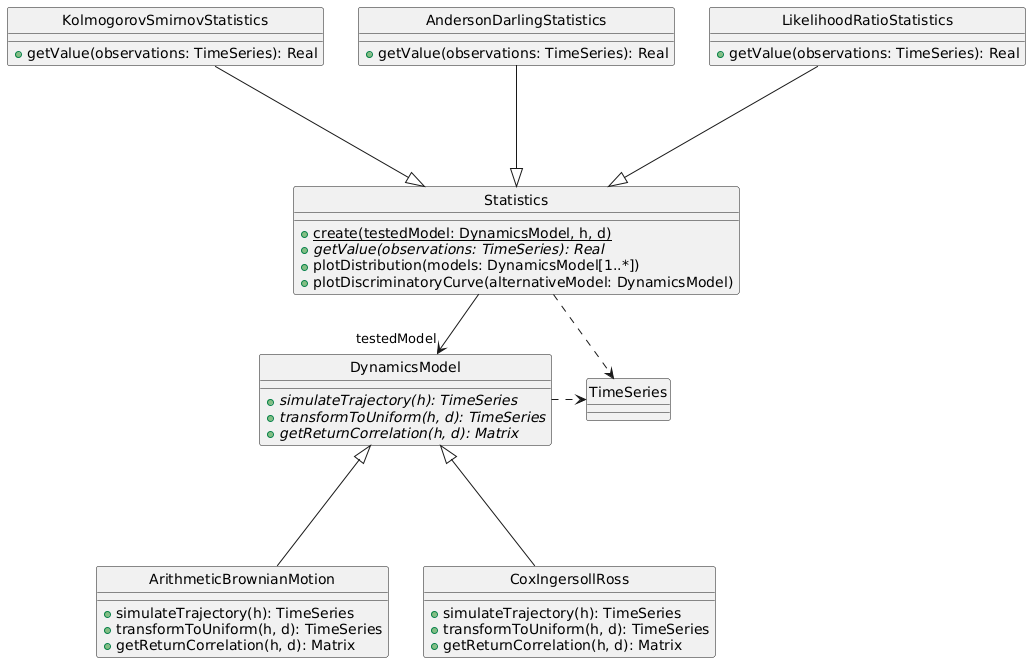
\includegraphics[width=0.9\linewidth]{uml.png}
    \caption{Дизайн проекта.}
    \label{fig:fft-heston-cpp}
\end{figure}

\section{Пайплайн проекта}

В ходе работы над проектом были последовательно выполнены следующие задачи:
\begin{itemize}
    \item Выбор темы проекта;
    \item Анализ и выбор архитектуры;
    \item Определение конечного результата;
    \item Работа над статьей и написание ноутбука \textit{ClaytonImplementation.ipynb};
    \item Расширение статьи и применение освоеного интсрументария к 
    модели Кокса-Ингерсолла-Росса;
    \item Написание библиотеки \textit{statisticslib};
    \item Проверена работоспособность библиотеки в файлах \textit{launchBM.ipynb} и 
    \textit{launchCIR.ipynb} для броуновского движения и процесса CIR соответсвенно;
    \item Была попытка ускорить программу с помощью переноса кода 
    симулятора траекторий броуновского движения. Был переписан код 
    файла \textit{ArithmeticBrownianMotion.py} на язык C++, но не удалось 
    применить swig для портирования на python;
    \item Настройка GitHub Actions для использования Doxygen;
    \item Оформление документации проекта.
\end{itemize}
В ноутбуке \textit{ClaytonImplementation.ipynb} были сохранены все оригинальные 
названия и обозначения из статьи, для удобства понимания. Однако при написании 
библиотеки \textit{statisticslib} мы пользовались принципами, изложенными в 
книге \cite{RMcode}, и обдумывали название каждой функции и переменной для 
удобного использования этой библиотеки.

\section{Реализация}

Имплементация статьи сделана в ноутбуке \textit{ClaytonImplementation.ipynb}, в котором 
шаг за шагом c \textbf{подробными комментариями} проделано то, 
что описано в \cite{Cl2019}.

Основные шаги имплементации:
\begin{itemize}
    \item Анализ содержания статьи: изучение подходов к бэктестингу моделей 
    прогнозирования волатильности;
    \item Реализация статистических гипотез: проверка гипотезы на принятие 
    или отвержение истинности гипотезы. Подробнее об этом можно 
    найти в \cite{Peres2004}.
    \item Использование корреляционной структуры: модификация статистических 
    тестов для учета корреляций в пересекающихся наблюдениях;
    \item Генерация графиков: построение визуализаций для демонстрации 
    мощности статистических тестов;
    \item Расширение моделей: применение методов статьи к более сложным 
    стохастическим моделям, выбранным и изученным по \cite{Sh2005}. 
\end{itemize}   

\section{Заключение}

В рамках проекта был реализован подход, описанный в статье \cite{Cl2019}, 
посвященный реализации методов по проверке гипотез о совпадении параметров 
двух коррелированных нормальных распределений. Итоговым результатом стала 
гибкая и готовая к дальнейшему использованию библиотека, разработанная на 
основе тщательно спроектированного дизайна.

Проект проиллюстрировал актуальность темы: использование 
скорректированных статистик для учета корреляционной структуры 
перекрывающихся наблюдений улучшает дискриминационную мощность тестов. 
Анализ открытых источников показал, что доступных реализаций этой 
статьи ранее не существовало.

Актуальность выбранной темы подчеркивается так же в недавней работе 
\cite{Piterb2023}, в которой были предложены новые методы исследований. 
Таким образом наш проект может быть расширен путем реализации 
описанных подходов, что повысит точность результатов.

\begin{thebibliography}{99}
    \bibitem{vega-cpp}
    Лекции и семинары по курсу \textit{"Программирование на C++ 
    для алгоритмической торговли и количественного анализа"}, 
    2024.
    \bibitem{Cl2019}
    \href{https://papers.ssrn.com/sol3/papers.cfm?abstract_id=3342541}
    {Michael A. Clayton, \textit{Backtesting Volatility Assumptions using 
    Overlapping Observations}, September 25, 2019.}
    \bibitem{RMcode}
    Роберт Мартин, \textit{Чистый код}, 2019.
    \bibitem{RMarch}
    Роберт Мартин, \textit{Чистая архитектура}, 2021.
    \bibitem{Sh2005}
    А.В. Булинский и А.Н.Ширяев, \textit{Теория случайных процессов}, 
    М.:ФИЗМАТЛИТ, 2005.
    \bibitem{Peres2004}
    Я.Р. Магнус, П.К. Катышев и А.А. Пересецкий, 
    \textit{Эконометрика}, 2004.
    \bibitem{Piterb2023}
    \href{https://papers.ssrn.com/sol3/papers.cfm?abstract_id=4571812}
    {Nikolai Nowaczyk, Vladimir Piterbarg \textit{Backtesting Correlated 
    Quantities}, September 13, 2023} 
    \end{thebibliography}

\end{document}
